\subsection{Griswold}
%Griswold
%Characteristics Dynamic language, Simple refactoring operations, Only One language, AST?, PDG?, Easy to create new operations?
Griswold \cite{griswold1991program} proved that meaning preseerving restructuring can substantively lower the cost of the maintenance of a system and improved the concept of restructuring by creating restructuring operations for the Scheme programming language implemented in Common Lisp. Scheme was chosen because of it's imperative features, simple syntax and it was available a PDG for scheme implemented in Common Lisp.


Griswold starts by comparing automated restructuring with manual restructuring using an experiment. It was presented to each subject an initial program and a description of the 4 goals of the transformations to do to that initial program and it was also asked to each subject to make sure that the modifications were correct, and to demonstrate that. 

Even though that they tested with a really small number of subjects, only 6, they managed to get several conclusions on how people manually restructure the programs.
People used a lot the Copy/Paste and the Cut/Paste paradigm to do the transformations, they copy or cut the code and then paste it in the desired location.
The Cut/Paste paradigm is more dangerous because if the user makes any error it is be more difficult to correct that error because it is a destructive operation.
This study also managed to conclude that people make mistakes even with simple and small programs and the cost of making mistakes is the time to do the restructuring.
One last conclusion was that manual restructuring is haphazard, the transformations were done in almost random way when compared to the computer-assisted process.


It was implement simple restructuring operations to prove the concept such as: Moving an expression, renaming a variable, in-lining/abstraction an expression, extracting a function, scope-wide function replacement, adding a reference indirection and adding looping to list references.


In order to be able to implement correctly this operations it was used contours and a PDG(program dependence graph). The main representation of the program is the contours that are an abstraction of the essential semantic properties that the AST represents in an efficient and complete form, but the PDG does not.
\begin{figure}[htbp]
  \centering
  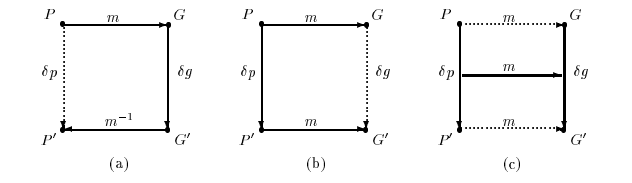
\includegraphics[width=0.95\textwidth]{img/Griswold1.png}
  \caption{Transformation diagrams (dotted arrows are implied mappings)}
  \label{fig:Griswold}
\end{figure}

$P$ represents the program in its core format (AST), while $G$ represents the PDG of the program.
$\delta$p is a function from source program to source programs P' using $\delta$p. 
({\bf Fig.~\ref{fig:Griswold} b}) shows the PDG G' being reconstructed from P' after $\delta$p is performed. 
This approach will be unacceptably time-consuming if $\delta$g is not performed. 
If both $\delta$p and $\delta$g exist then each representation can be updated by its own transformation procedures, yielding efficient updating for both the AST and the PDG. ({\bf Fig.~\ref{fig:Griswold} c})

One way to use the PDG is to translate the program into it’s PDG form, perform the transformation and then convert it back to it’s program form ({\bf Fig.~\ref{fig:Griswold} a}). this allows the use of the nice mathematical properties of the PDG for reasoning about the correctness of the implementation of the transformation function, as well as for the efficient application of semantically-oriented algorithms. However this approach would be unacceptably time-consuming if $\delta$g is not performed. 
With contours and a way to relate components in the PDG and the AST it is possible to combine then and have a single formalism to reason effectively about flow dependencies and scope structure.

%It is possible to have this representation because it have access to everything like a compiler does, and it tries to used work done, such as using a library for the PDG. Using DrRacket the semantic part is covered by the arrows created which helps having the semantic logic between things.
